\documentclass[4pt,a4papper]{article}
\usepackage{ctex}  
\usepackage{amsmath}
\usepackage{mathtools}
\usepackage{upgreek}
\pagestyle{headings}
\usepackage{graphicx}
\usepackage{subfigure}
\usepackage{indentfirst}
\usepackage{fancyhdr}
\usepackage{listings}
\usepackage{amsmath}
\usepackage{longtable}
\usepackage{geometry}
\usepackage[usenames,dvipsnames]{color}
\definecolor{lightgray}{RGB}{230,230,230}
\lstset{ language=, numbers=left, basicstyle=\small,
  keywordstyle=\color{blue}, commentstyle=\color{PineGreen},
  stringstyle=\color{red}, frame=shadowbox, breaklines=true,
  backgroundcolor=\color{lightgray},extendedchars=false }


\geometry{left=2.0cm,right=2.0cm,top=2.5cm,bottom=1.5cm}

%opening
\title{\zihao{-2}\textbf{丙酮碘化实验报告}}
\author{张锦程}
\date{\today}

\begin{document}
\maketitle
%\tableofcontents

\section{\zihao{4}实验目的}
1. 采用分光光度法测定用酸作催化剂时丙酮碘化反应的速率系数、反应级数和活化能。 

2. 通过本实验加深对复合反应特征的理解。 

3. 熟练掌握分光光度计的原理和使用方法。

\section{\zihao{4}实验原理}
	大多数化学反应并不是简单反应(只含一个基元反应),而是由若干个基元反应组成的复合反应。大多数复合 反应的反应速率和反应物浓度间的关系较为复杂(非质量作用定律)。测定这些反应对各组分的分级数,从而得到 复合反应的速率方程,是反应动力学的重要内容,而当我们知道反应速率方程的形式后,就可以对反应机理进行一 定推测。如该反应究竟由哪些步骤组成,各步骤的特征和相互联系如何等。

	酸性溶液中,丙酮碘化反应是一个复合反应,其反应式为:$(CH_3)_2CO + I_3^- → CH_3COCH_2I + H^+ + 2I^-$ ; 其速率方程为:$r = kc^\alpha(A)c^\beta(I_3^-)c^\delta(H^+)$ 

	$I_3^-$ 在可见光区有一个比较宽的吸收带,而在这个吸收带中,盐酸和丙酮没有明显的吸收,所以可以使用分光光度计,通过测定光密度的变化来测定 $I_3^-$ 浓度的变化,以跟踪反应过程。但 I2 的存在会对实验产生干扰,总消光度 $D = D(I_3^-) + D(I_2) = ε(I_3^-)LC(I_3^-) + ε(I_2)LC(I_2)$; 在 565nm 这一特定波长条件下, $ε(I_3^-) = ε(I_2);D = D(I_3^-) + D(I_2) = ε(I_3^-)L[C(I_3^-) + C(I_2)]$ 

	在本实验条件下,实验将证明丙酮碘化反应对碘是零级反应,即 $β=0$。由于反应并不停留在一元碘化丙酮上, 还会继续进行下去,因此反应中所用的丙酮和酸的浓度应大大过量。而所用的碘量很少。这样,当少量的碘完全消 耗后,反应物丙酮和酸的浓度可以认为基本保持不变。此时, $r = \frac{-dc(I_3^-)}{dt} = kc^\alpha(A)c^\delta(H^+) = const$

	显然,为了测定反应级数,例如指数 $\alpha$,至少需进行两次实验。在两次实验中丙酮的初始浓度不同,$H^+$ 和 $I_3^-$ 的初始浓度相同, $\frac{r_I}{r_{II}} = [c^\alpha(A,I)c^\delta(H^+,I)]/[c^\alpha(A,II)c^\delta(H^+,II)] = u^\alpha$;取对数得:$\alpha= \frac{lg(\frac{rI}{rII})}{lgu}$ ;同理可求指数$\delta,\beta$ 进一步,由两个或两个以上温度的速率系数,根据阿累尼乌斯公式:$k = Ae^{-\frac{Ea}{RT}}$,可以估算反应的表观活化能 $E_a$ 。

\section{\zihao{4}实验操作}
1、 检查仪器和药品。

2、 接通电源,开启恒温槽,检查水路是否通畅和漏水。将装入已标定好的碘溶液、丙酮溶液、盐酸溶液的玻璃瓶 放入恒温槽中恒温。恒温槽温度设定在 25℃。到达设定温度并恒定 10 分钟后开始实验。 

3、 打开分光光度计电源开关,波长调至 565nm,预热一段时间后放入装有已恒温的去离子水的比色皿, 作为空白调零。

4、 测定εL 值。准确移取 2.5ml 碘溶液于 25ml 容量瓶中,用已恒温的去离子水稀释至刻度,摇匀,润洗比色皿 3 次,然后将装有 2/3 溶液的比色皿置于样品室光路通过处,盖好盖子。更换碘溶液再重复测定两次,取其平均值求ε

5、 测定四种不同配比溶液的反应速度,配比如下:

\begin{table}[htbp]
\centering
\begin{tabular}{|l|l|l|l|}
\hline
         & 碘溶液 V/mL & 丙酮溶液 V/mL & 盐酸溶液 V/mL \\ \hline
I(25℃)   & 5        & 5         & 5         \\ \hline
II(25℃)  & 5        & 2.5       & 5         \\ \hline
III(25℃) & 5        & 5         & 2.5       \\ \hline
IV(25℃)  & 7.5      & 5         & 5         \\ \hline
V(35℃)   & 7.5      & 5         & 5         \\ \hline
\end{tabular}
\end{table}




\section{\zihao{4}实验结果讨论}
\subsection{\zihao{-4}计算过程}
1. 根据所测已知碘浓度的光密度用 $D = \epsilon Lc$ 计算出常数 $\epsilon (I_3^-)L$ 值。然后用它们计算与所测得的每个光密度值相应的碘浓度 $c(I_3^-)$,作 $c(I_3^-) - t$ 图,求出反应速率 $r$
 
2. 根据 $\alpha= \frac{lg(r_I/r_{II})}{lgu}$ 等式子分别计算对丙酮、盐酸和碘的分级数。 

3. 根据 $r = kc^\alpha(A)c^\beta(I_3^-)c^\delta(H^+)$ 计算 25℃时丙酮碘化反应的四个速率系数。求出 $k_1$ 的平均值。计算 35℃时的速率系数 $k_2$。

4. 利用阿累尼乌斯公式求出丙酮碘化反应的表观活化能 $E_2$


\subsection{\zihao{-4}原始数据}
\subsubsection{\zihao{5}溶液原始浓度}
\begin{table}[htbp]
\begin{tabular}{|l|l|l|l|}
\hline
溶液原始浓度     & 碘溶液浓度  & 丙酮溶液浓度 & 盐酸浓度   \\ \hline
浓度值(mol/L) & 0.0195 & 2.5000 & 0.8670 \\ \hline
\end{tabular}
\end{table}
\subsubsection{\zihao{5}碘溶液的吸光度}
\begin{table}[htbp]
\begin{tabular}{|l|l|l|}
\hline
碘溶液(0.0195mol/L) & 吸光度      & 透过率      \\ \hline
数值               & 0.342861 & 45.40868 \\ \hline
\end{tabular}
\end{table}
\subsubsection{\zihao{5}仪器常数$\epsilon L$}
$\epsilon L = \frac{A}{c(I_2)+c(I_3^-)} = \frac{0.342861}{0.001950} = 175.826 L/mol$


\subsection{\zihao{-4}计算结果}
由于反应开始时温度不稳定可能导致结果偏低,本实验取数据的后 $\frac{1}{3}$ 段进行线性拟合,并由斜率求得反应速率,不同浓度时的计算结果如下图所示:

    \begin{figure}[htb]
        %\small
        \centering
        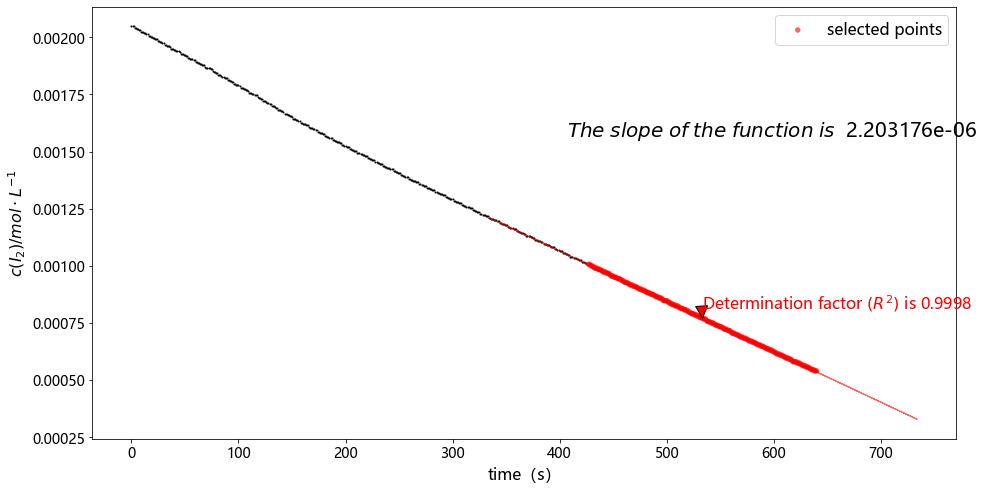
\includegraphics[width=15cm]{./figures/5;5;5.png}
        \caption{5mL 碘,5mL 丙酮,5 mL 盐酸,25℃} \label{fig: 1}
    \end{figure}
~\\
~\\
    \begin{figure}[hb]
        %\small
        \centering
        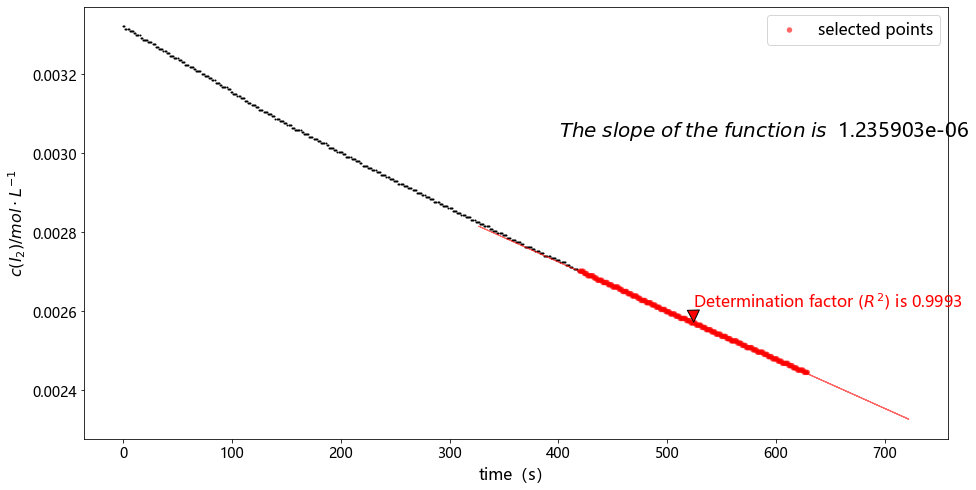
\includegraphics[width=15cm]{./figures/5;2.5;5.png}
        \caption{5mL 碘,2.5mL 丙酮,5 mL 盐酸,25℃} \label{fig: 2}
    \end{figure}

\newpage

    \begin{figure}[htp]
        %\small
        \centering
        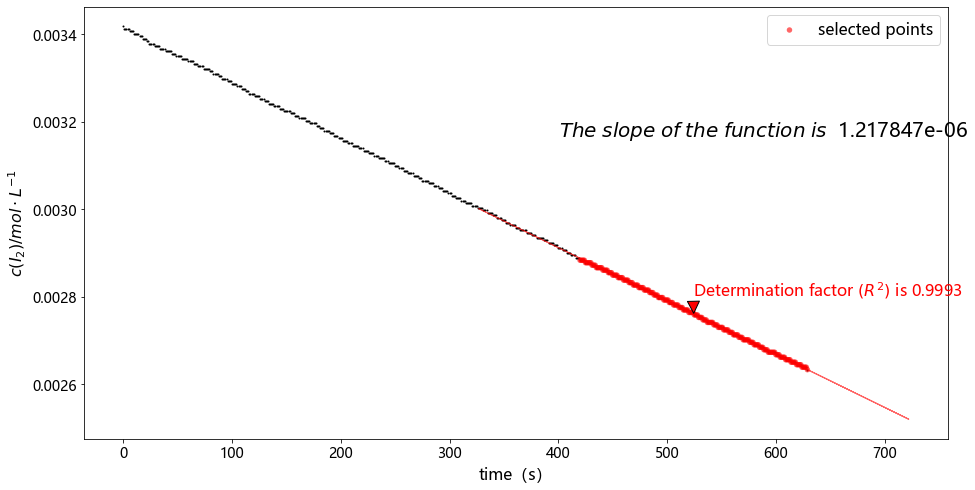
\includegraphics[width=15cm]{./figures/5;5;2.5.png}
        \caption{5mL 碘,5mL 丙酮,2.5 mL 盐酸,25℃} \label{fig: 3}
    \end{figure}
~\\
~\\
    \begin{figure}[hbp]
        %\small
        \centering
        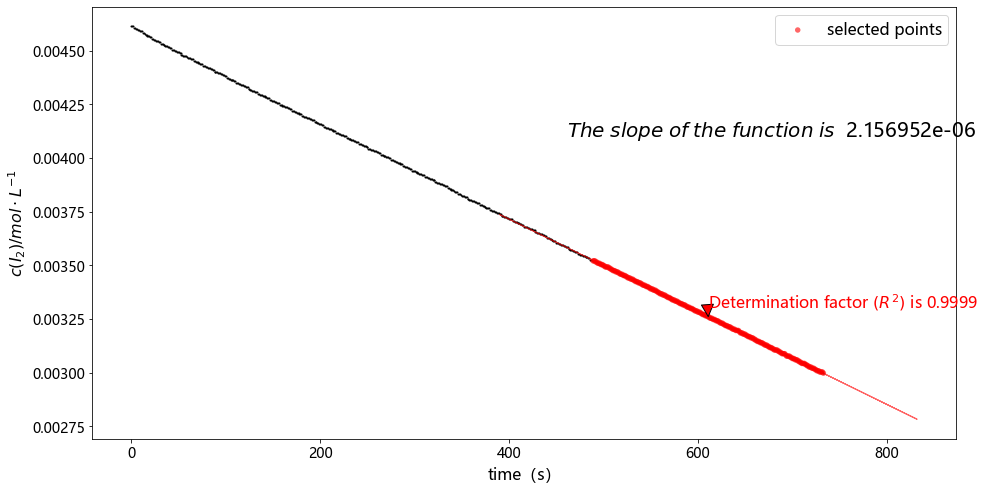
\includegraphics[width=15cm]{./figures/7.5;5;5.png}
        \caption{7.5mL 碘,5mL 丙酮,5 mL 盐酸,25℃} \label{fig: 4}
    \end{figure}

\newpage
    \begin{figure}[htp]
        %\small
        \centering
        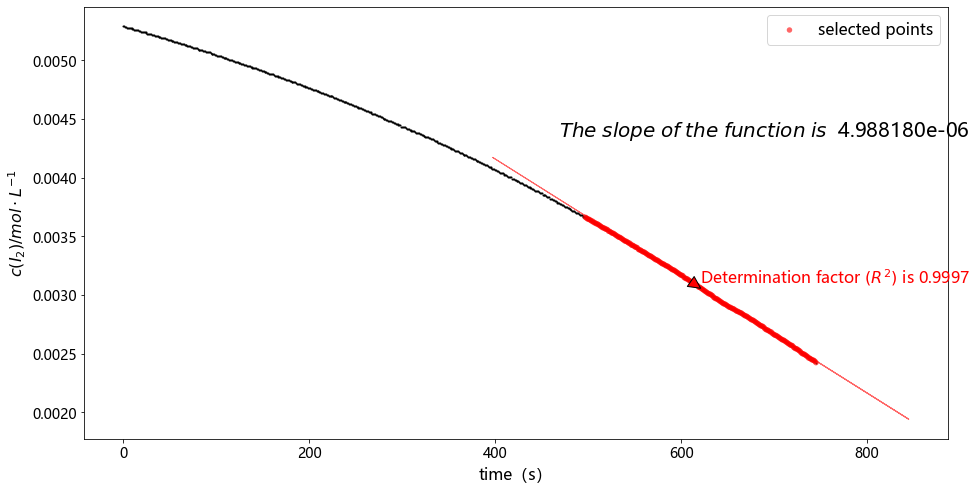
\includegraphics[width=15cm]{./figures/7.5;5;5;35C.png}
        \caption{7.5mL 碘,5mL 丙酮,5 mL 盐酸,35℃} \label{fig: 5}
    \end{figure}


整理得下表:
\begin{table}[htbp]
\centering
\begin{tabular}{|l|l|l|l|l|}
\hline
溶液原始浓度   & 碘溶液 V/mL & 丙酮溶液 V/mL & 盐酸浓度 V/mL & 反应速率/ $\mu mol\cdot L^{-1}\cdot s^{-1}$ \\ \hline
I (25℃)   & 5        & 5         & 5         & 2.203                                     \\ \hline
II(25℃)  & 5        & 2.5       & 5         & 1.236                                     \\ \hline
III(25℃) & 5        & 5         & 2.5       & 1.218                                     \\ \hline
IV(25℃)  & 7.5      & 5         & 5         & 2.157                                     \\ \hline
V (35℃)   & 7.5      & 5         & 5         & 4.988                                     \\ \hline
\end{tabular}
\end{table}



由表中数据可得:

$$
\alpha = \frac{ln(r_I/r_{II})}{ln(c(A)_I/c(A)_{II})} = \frac{ln(2.203/1.236)}{ln(5/2.5)} = 0.834
$$
$$
\beta = \frac{ln(r_I/r_{IV})}{ln(c(I_2)_I/c(I_2)_{IV})} = \frac{ln(2.203/2.157)}{ln(5/7.5)} = -0.052
$$
$$
\delta = \frac{ln(r_I/r_{III})}{ln(c(H^+)_I/c(H^+)_{III})} = \frac{ln(2.203/1.218)}{ln(5/2.5)} = 0.855
$$

~\\

由 $r = kc^\alpha(A)c^\beta(I_3^-)c^\delta(H^+)$ 计算 25℃ 时丙酮碘化反应的四组速率系数分别为:

\begin{table}[htbp]
\centering
\begin{tabular}{|l|l|l|l|l|}
\hline
速率系数 k & 0.1580 & 0.1581 & 0.1581 & 0.1581 \\ \hline
\end{tabular}
\end{table}

求出 $k_1$ 的平均值为:0.1581;同理计算出 35℃ 时的速率系数 $k_2$ 为:0.3655

利用阿累尼乌斯公式 $ln(\frac{k_1}{k_2}) = -\frac{E_a}{R}(\frac{1}{T_1} - \frac{1}{T_2})$ 求出丙酮碘化反应的表观活化能 $E_2$ 为: 63970.869 J
\newpage


\section{\zihao{4}附录}
\subsection{\zihao{-4}思考题}
1. 在动力学实验中,正确计量时间是很重要的。本实验中从反应开始到起算反应时间,中间有一段不 算很短的操作时间。这对实验结果有无影响?为什么?

	影响不大,因为本反应为 0 级反应,I2浓度的下降是线性的,所以只要在实验中存在一段平直的反应曲线,就可以 测出反应速率,和初始状态无关

2. 影响本实验结果的主要因素是什么? 

	主要是要控制反应温度的恒定,反应具有热效应,可能导致温度变化,从而影响到所测得的反应速率

3. 如果用表观活化能 Ea 代替活化焓Δ≠Hm 行否?为何? 

	不行,它们之间差了一个 RT 项,当活化能较小时,会存在误差



\clearpage
\end{document}